\documentclass[brainsci,article,submit,moreauthors]{Definitions/mdpi}

\firstpage{1}
\makeatletter
\setcounter{page}{\@firstpage}
\makeatother
\pubvolume{1}
\issuenum{1}
\articlenumber{0}
\pubyear{2026}
\copyrightyear{2026}
\datereceived{ }
\daterevised{ }
\dateaccepted{ }
\datepublished{ }

\Title{Visual Perception Changes as the Etiology of Sundowning Syndrome}

\Author{Erbil Can Artun $^{1}$ and Afif Siddiki $^{2,3,}$*}

\AuthorNames{Erbil Can Artun and Afif Siddiki}

\address{%
$^{1}$ \quad T\"UB\.ITAK National Metrology Institute (UME), Gebze, Kocaeli 34083, Turkey\\
$^{2}$ \quad Atlas University Vocational School, Anadolu Cd. No. 40, Hamidiye, \.Istanbul 34408, Turkey\\
$^{3}$ \quad Institute for Solid-State Electronics, Leibniz Institute in the Research Association Berlin e.V., Hausvogteiplatz 5--7, 10117 Berlin, Germany}

\corres{Correspondence: afif.siddiki@atlas.edu.tr}

\abstract{\textbf{Background/Objectives:} The literature describes sundowning syndrome as a peculiar anxiety behaviour of elderly humans during the late afternoon or early evening period. But such an uneasy feeling is also common among ordinary people at this time. In this paper we present a model that, using basic physics, evolutionary biology and psychiatric knowledge, offers a potential explanation for this everyday observation in our lives. \textbf{Methods:} Possible causes of this syndrome are investigated by the changes in visual perception in dependence on solar radiation and its wave properties. We briefly review relevant astronomical principles and biological aspects of vision. Then, we show that visual perception depends on solar time. \textbf{Results:} We show quantitatively that the solar-time dependence of vision is consistent with the reported time window of clinical sundowning observations. \textbf{Conclusions:} The shift from photopic to scotopic vision at twilight may be a physical cue for sundowning behaviour, and plotting its timing with latitude and season indicates tailored ambient lighting protocols as a potential~intervention.}

\keyword{sundowning syndrome; Alzheimer's disease; dementia; circadian rhythm; visual perception; mesopic vision; photoreceptors; solar radiation}

\begin{document}

\section{Introduction}

In many languages, songs or poems that stress the particular sadness of the artist at sunset and at autumn are common. These are periods when this sort of uneasiness may be observed in ourselves or in mentally healthy persons around us. Such mood change over time is studied clinically in patients with Alzheimer's and dementia \citep{martin2000,gallagher1992}.

Scientific progress has resulted in enormous advances in industrial and agricultural production and in medical sciences. Such improvements lead to a longer life expectancy of human beings. Consequently, the number of older people has increased remarkably \citep{oecd2020}. Dementia \citep{who2017} is one of the most well-known health problems in older adults. It is a broad term used to describe cognitive impairment, which is a decline in mental abilities such as orientation, language, and reasoning. Alzheimer's disease is named after Dr. Alois Alzheimer, who observed some abnormal physiological anomalies in the brain autopsy of his patient in 1906 \citep{nih2019}. Since then, there has been debate about the causes and treatment of this disease \citep{burns2009,larson2013}. Sundowning syndrome (SS) is a poorly understood but interesting phenomenon in Alzheimer's patients (AP), described as sudden and abnormal behavioural changes including depression, agitation, disorientation, etc., and it is observed quite often (2.4\%--66\%) in late afternoon or early evening \citep{martin2000,gallagher1992}. Many APs have been reported to show abnormal behaviour (e.g., agitation, disorientation, etc.) during the late afternoon or early evening \citep{khachiyants2011}. The sundowning syndrome is explained by several proposed mechanisms such as perceptual disorders \citep{martin2000,khachiyants2011} and changes in circadian rhythms \citep{cohenmansfield1989} that are more directly related to light exposure, among other well-studied reasons \citep{khachiyants2011}.

From the literature given above, it can be seen that even if one assumes that SS comes from light exposure, it is not clear how this is related to time and even the location of the patients. We know that the Sun is shining and the Moon is shining. We have less sunshine in the winter than we do in the summer. Interestingly, the change from day to night within the framework of visual perception has not been discussed in the literature within the framework of SS. The effect of light change on this syndrome is still debated, but most recent investigations strongly support the light-dependent proposal. The scheme of calculation is offered on the basis of ideas of astronomy, electromagnetic and quantum theories, and also evolutionary biology and visual physiology. Our model explains the association of the sundowning syndrome with daytime light exposure from solar irradiation, taking into account also visual physiology.

Finally, we close our paper by discussing the clinical implications of our approach.

\begin{figure}[H]
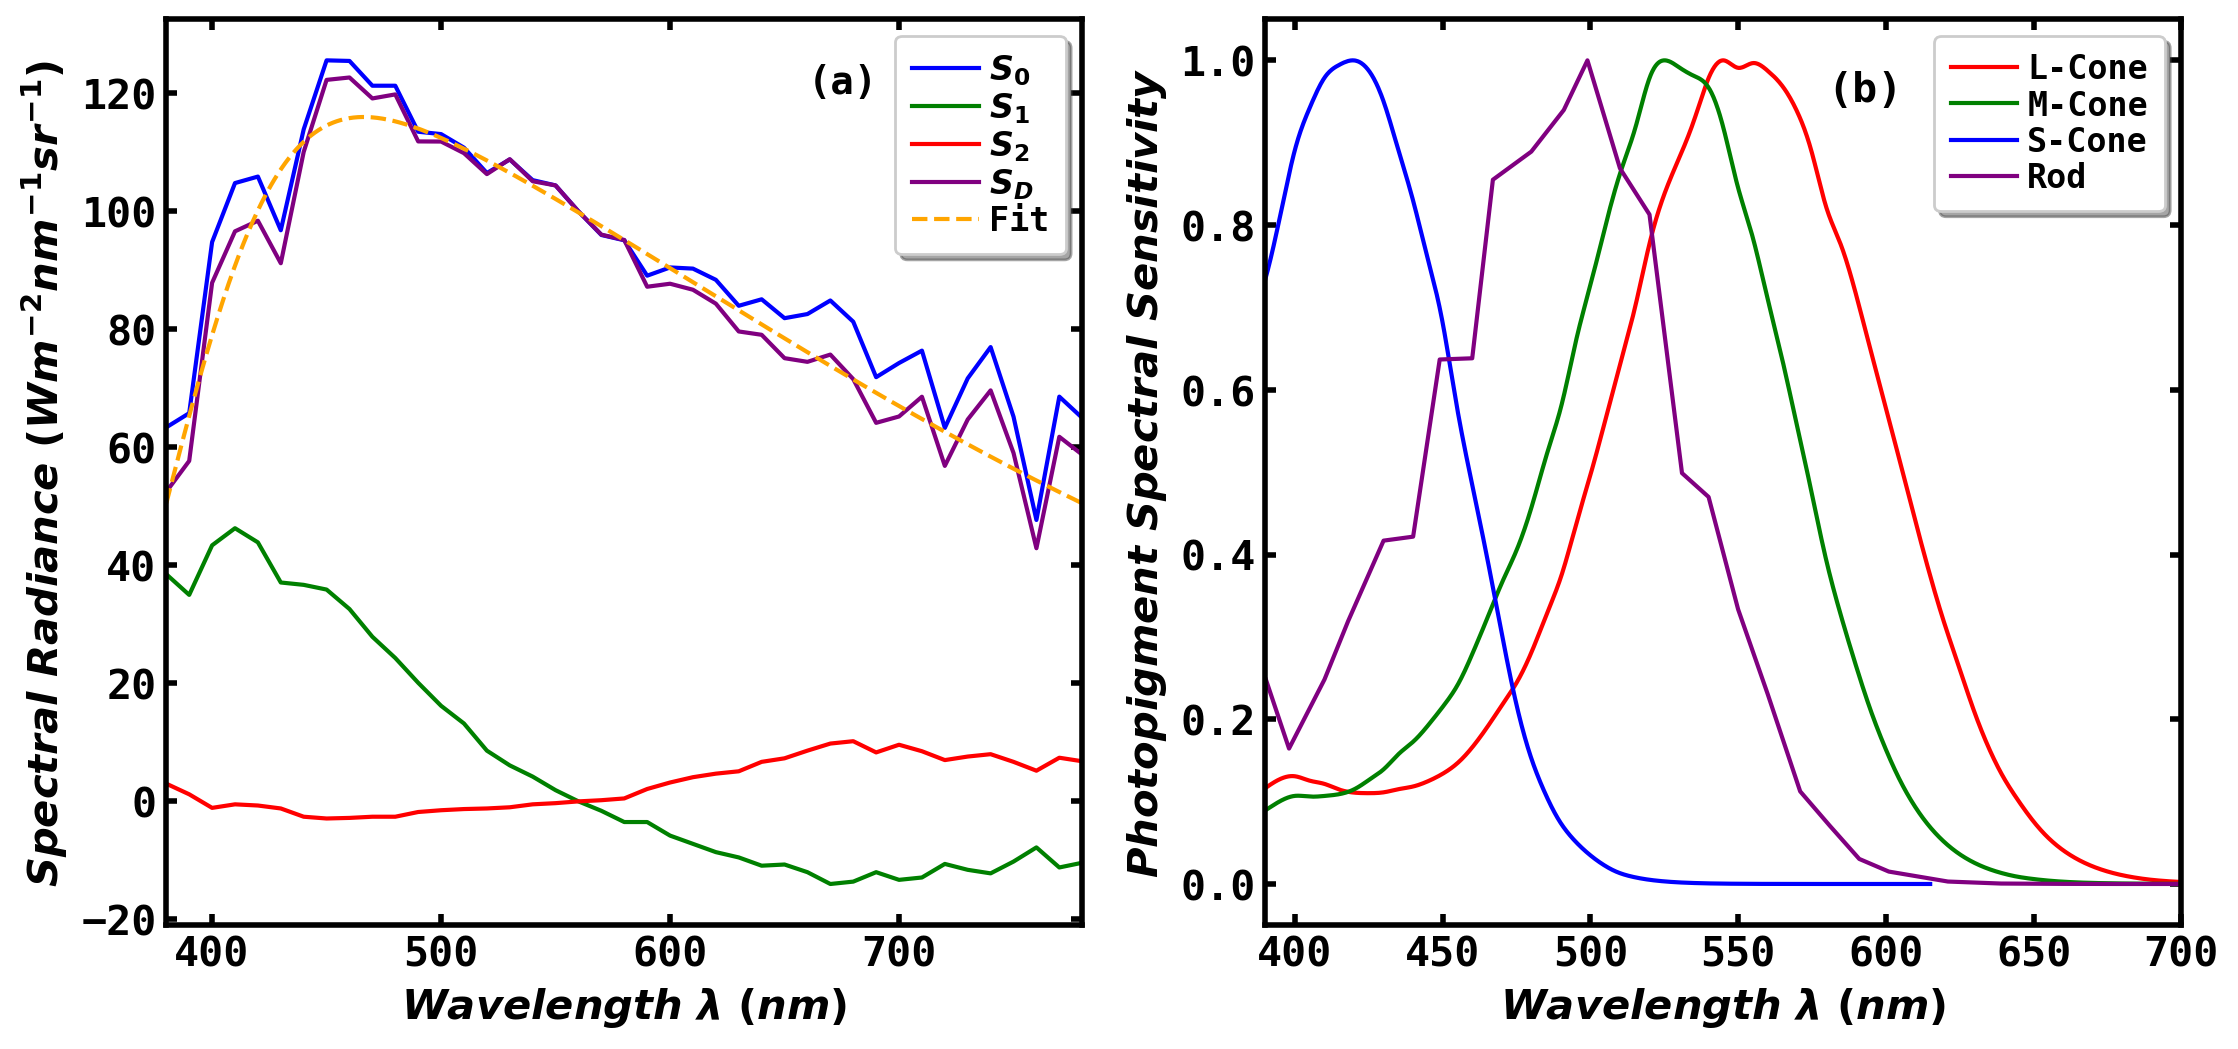
\includegraphics[width=\linewidth]{figure1}
\caption{(\textbf{a}) Solar radiation spectra at a given time and location (29 October 2023, Ankara, Turkey) including the scattering from the atmosphere. The dashed line is a fit to a Planck blackbody spectrum. (\textbf{b}) Spectral sensitivity of the rod (magenta) and cone (blue---S, green---M and red---L) cells.\label{fig1}}
\end{figure}
\unskip

\section{Results and Discussion}

It is one of the most complicated machineries we have: our brain and its mutual extension, our eyes, and their structure and properties are such. Certainly, some animals have much better visual functions than ours under certain conditions. But the human brain has vastly greater data-processing capabilities than other animals. Indeed, our visual and other faculties are almost entirely dependent on our environment. From the point of view of vision, the Sun is the main actor. Figure~\ref{fig1}a shows the solar spectrum as a function of wavelength. The data shown are from the NASA archive, with the dashed line being the fit of Planck's black-body spectrum. Here, $S_{0}$, $S_{1}$ and $S_{2}$ are the scattered light intensities and $S_{D}$ is the point light intensity of the viewer \citep{preetham1999}. The calculation scheme is briefly summarised in the Materials and Methods section.

Our eyes have two parts, in which two types of vision cells reside. The retina is the inner surface of the eye. The fovea is at the centre of that surface. Cells that respond to black and white are called scotopic (rod) cells and those that respond to colour are photopic (cone) cells. Most photopic cells are in the fovea, while scotopic cells are mainly in the retina. The electrochemical behaviour of these cells at the molecular scale is very well understood \citep{boynton1979}. Light (a photon) hitting molecules in the cells (rhodopsin, for example) changes the conformation of the molecule and generates an electrical signal which is sent to the brain via the optical nerves.

Interestingly, scotopic and photopic cells are quite different in their sensitivity to the light intensity and wavelength. At low wavelengths ($\lesssim 500$~nm, bluish) scotopic cells dominate over photopic cells, which helps us see better in the dark. Photopic cells are more sensitive to higher wavelengths ($\gtrsim 530$~nm, red). Another difference is their maximum sensitivity, which depends on the intensity and wavelength. These differences are shown in Figure~\ref{fig1}b. The two observations above account for why we see red better in the daytime and blue at night. It is also understandable from an evolutionary point of view, because cone sensitivity is highest in the yellow-green region in daylight, where the solar spectrum at the surface also peaks. In dim light the sensitivity shifts to the blue-green region \citep{boynton1979}.

The right panel of Figure~\ref{fig1} shows the sensitivity of our eye cells as a function of wavelength, for both rod (magenta) and cone (blue, green and red) cells, reproduced from Refs.~\citep{kraft1993,schnapf1987}. The rod cells are more sensitive to blue-green light (480--520~nm). Meanwhile, cone cells are specialised for short (S, blue), medium (M, green) and large (L, red) wavelengths. In the red colour interval ($\sim$652--740~nm) only the L-cone cells are sensitive. When we come to consider the effect of visual perception during the late afternoon and early evening, the insensitivity of our eyes to red colour will become more important. The sensitivities of the cone cells are taken from Ref.~\citep{stockman1993}.

From the sky we can calculate the amount of light that reaches our eyes and get the visual perception as a function of time. One must also calculate how much light is received by our rod and cone cells. In the following, we will use these physiological findings together with physics-based formulations to calculate day-dependent visual abilities. In an effort to address the main motivation of our study, the sundowning syndrome, we analyse the time periods when the vision switches from photopic to scotopic.

Time, in essence solar time, is vital in the biological machinery that we inherited from evolution. Recent studies on circadian time of cells, tissues, plants, animals and human beings, even at the level of genetic heritage, have made remarkable breakthroughs in our understanding of living organisms \citep{cao2021}.

Our approach is based on the accurate determination of the human (total) vision as a function of time and location. We then analyse changes in vision as a function of scotopic (rod, luminance sensitive) and photopic (cone, colour sensitive) cells. We finally show that there is a turning point of total vision, which depends not only on the day, but also on the place and the clearness of the sky.

By using well-developed astronomical methods and visualisation techniques, changes in vision depending on environmental conditions \citep{preetham1999} are calculated by the Sun's irradiance on the Earth. But before analysing the physiology of vision in terms of the properties of visual cells, we should again consider the intensity of the visible light emitted by the Sun as a function of the wavelength, in view of the blackbody radiation and the atmospheric attenuation, i.e., the Rayleigh scattering. Hence, we will, for future convenience, call visible light simply light. During the daytime, the sky is blue, but during sunrise or sunset, it turns reddish. For the rest of the time, the sky is black, i.e., no light (visible electromagnetic radiation from the Sun) is seen.

The molecules that make up the atmosphere are mostly nitrogen and oxygen, so when sunlight hits our Earth, these molecules scatter it. They scatter short (blue) wavelengths much more efficiently than long ones, so the scattered blue light comes to the observer from all directions in the sky. So we have a blue sky. At sunrise and sunset, the light has to travel a longer distance through the atmosphere, and most of the short-wavelength (blue) light is scattered out of the line of sight, so the light that is directly transmitted is dominated by longer (red) wavelengths. After sunset (before sunrise), we see that the sky turns black.

Next, we should note that the Sun does not radiate equally well at all wavelengths. Wavelengths close to blue are more dominant than other colours, and low-energy wavelengths like red are emitted less. Max Planck first explained the intensity of radiation from stars as a function of temperature and wavelength, which actually gave rise to quantum mechanics \citep{shankar1994,griffiths2017}.

\begin{figure}[H]
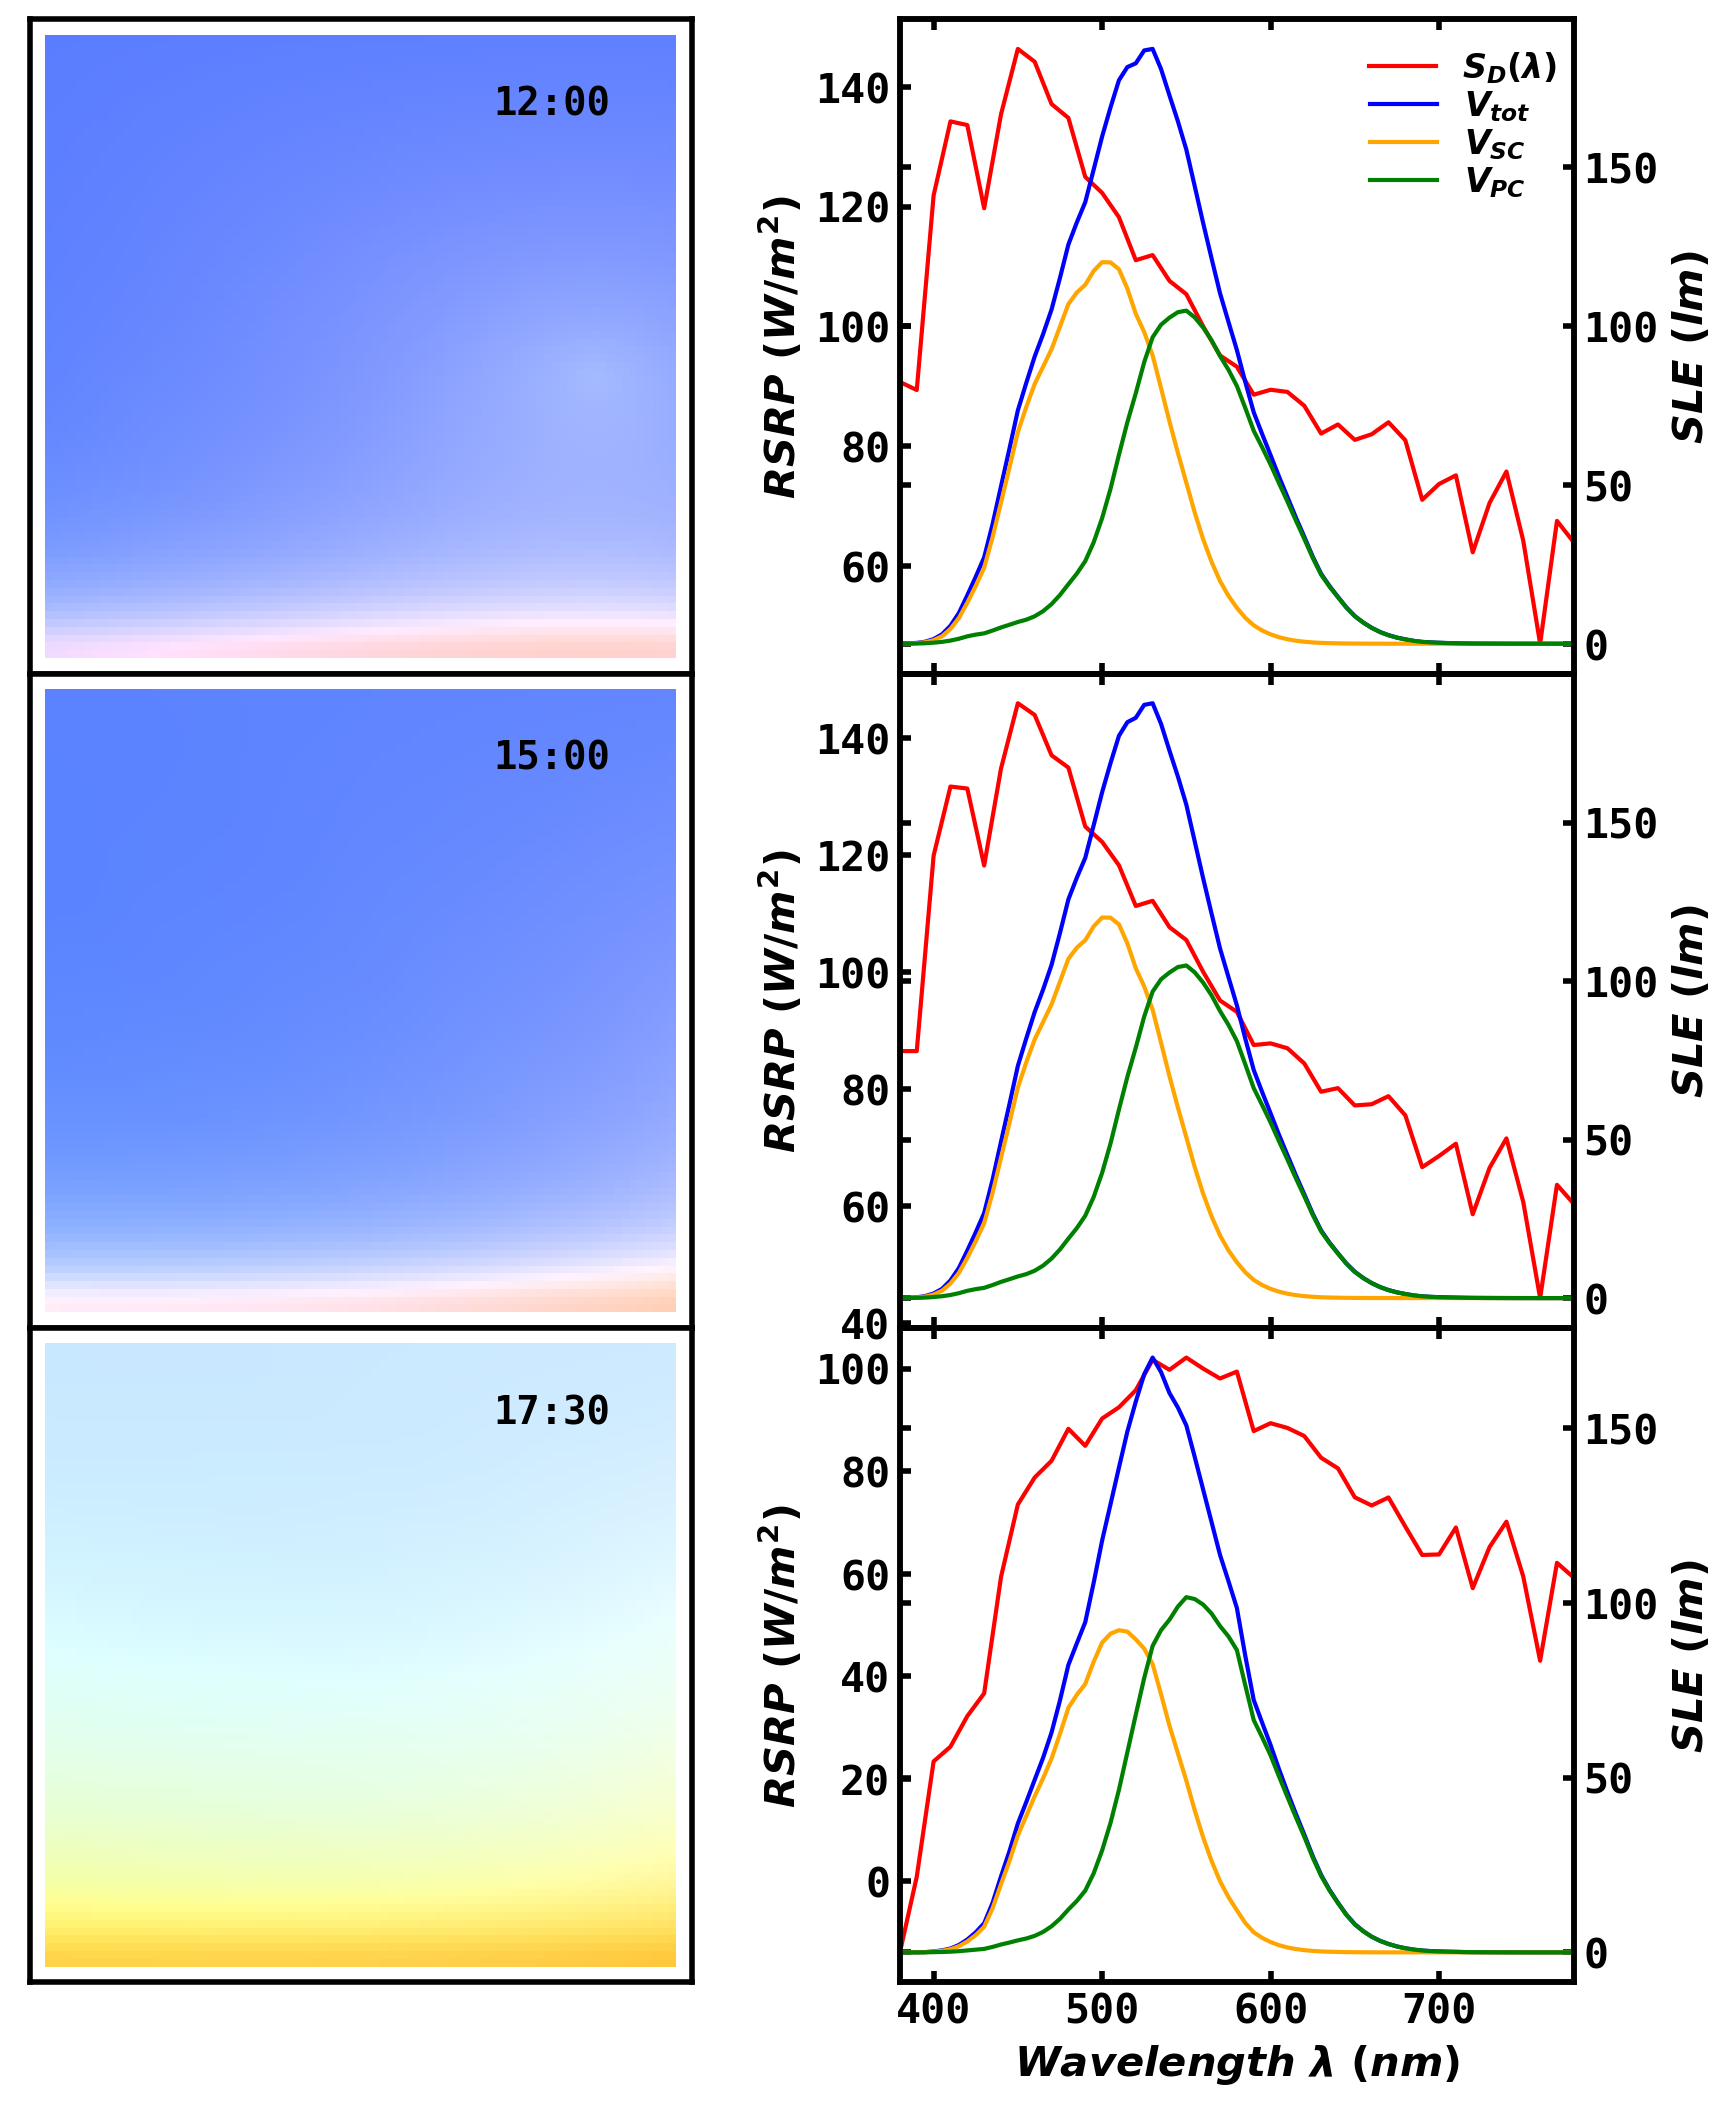
\includegraphics[width=\linewidth]{figure2}
\caption{(\textbf{Left panel}) The colour of the sky in Ankara at three characteristic times. (\textbf{Right panel}) Corresponding sky spectral radiance density with scotopic (yellow), photopic (green), and total vision (blue).\label{fig2}}
\end{figure}
\unskip

With the above discussions and approaches, the light intensity as a function of time of day and year, and wavelength, for a given location can be quantitatively obtained. We have not included the climate, and we have always adopted a very clear sky with a turbidity of 2. As an example of the sky colour, see Figure~\ref{fig2} (left panel), calculated from the mathematical formulation given in Ref.~\citep{preetham1999} and visualised by our computational methods. Here we consider the location of Ankara, Turkey (lat. $39.90^{\circ}$~N, long. $32.800^{\circ}$~E, and altitude 938~m). Due to the turbidity the horizon is a little reddish and the sky is white-blueish at 12:00 and 15:00. Later, at sunset, the horizon is orange-reddish and the sky is more and more turquoise. It is the usual view of the sky at most mid-latitude places in the northern hemisphere, that is, above the Tropic of Cancer. In the right panel of Figure~\ref{fig2} we plot the sky light spectra (red) together with the scotopic (yellow), photopic (green) and total vision as a function of wavelength. One can see the change of the spectrum of the sky with time and also its effect on total vision. In the two upper panels scotopic vision is dominant, in the lower panel photopic vision dominates total vision.

As we have pointed out in the introduction, we often experience a mood of sadness-uneasiness at times approaching sunset or after solar noon. But there are some cases when these feelings might get more serious. Experts usually divide the severity of this feeling into sadness-uneasiness vs. depression-anxiety. Depression-anxiety is a psychiatric diagnosis. There is no quantitative conclusion in the literature, but it is generally accepted that the largest part of the individuals feel sadness-uneasiness for limited time intervals and with limited intensity. In contrast, anxiety-depression is prolonged in time, and these feelings begin to dominate the daily life of individuals, with potentially serious clinical and social consequences.

Sundowning syndrome is a medically investigated and reported abnormality of mood change during daytime. Patients present with aggression, regression, depression or anxiety. Is this change of mood anxiety, depression or delirium? This is still debated. So far as we know, it is still called a syndrome. However, patients suddenly behave differently than the rest of the day when time evolves from noon to evening. There are reliable clinical studies, published in the literature, explaining the mechanisms of these abnormal patient activities, mainly seen in elderly patients. It is important to understand the cause of such a behavioural change, as the proportion of elderly persons in modern societies is unprecedented in history and sundowning imposes a large burden on patients, caregivers and health systems.

\begin{figure}[H]
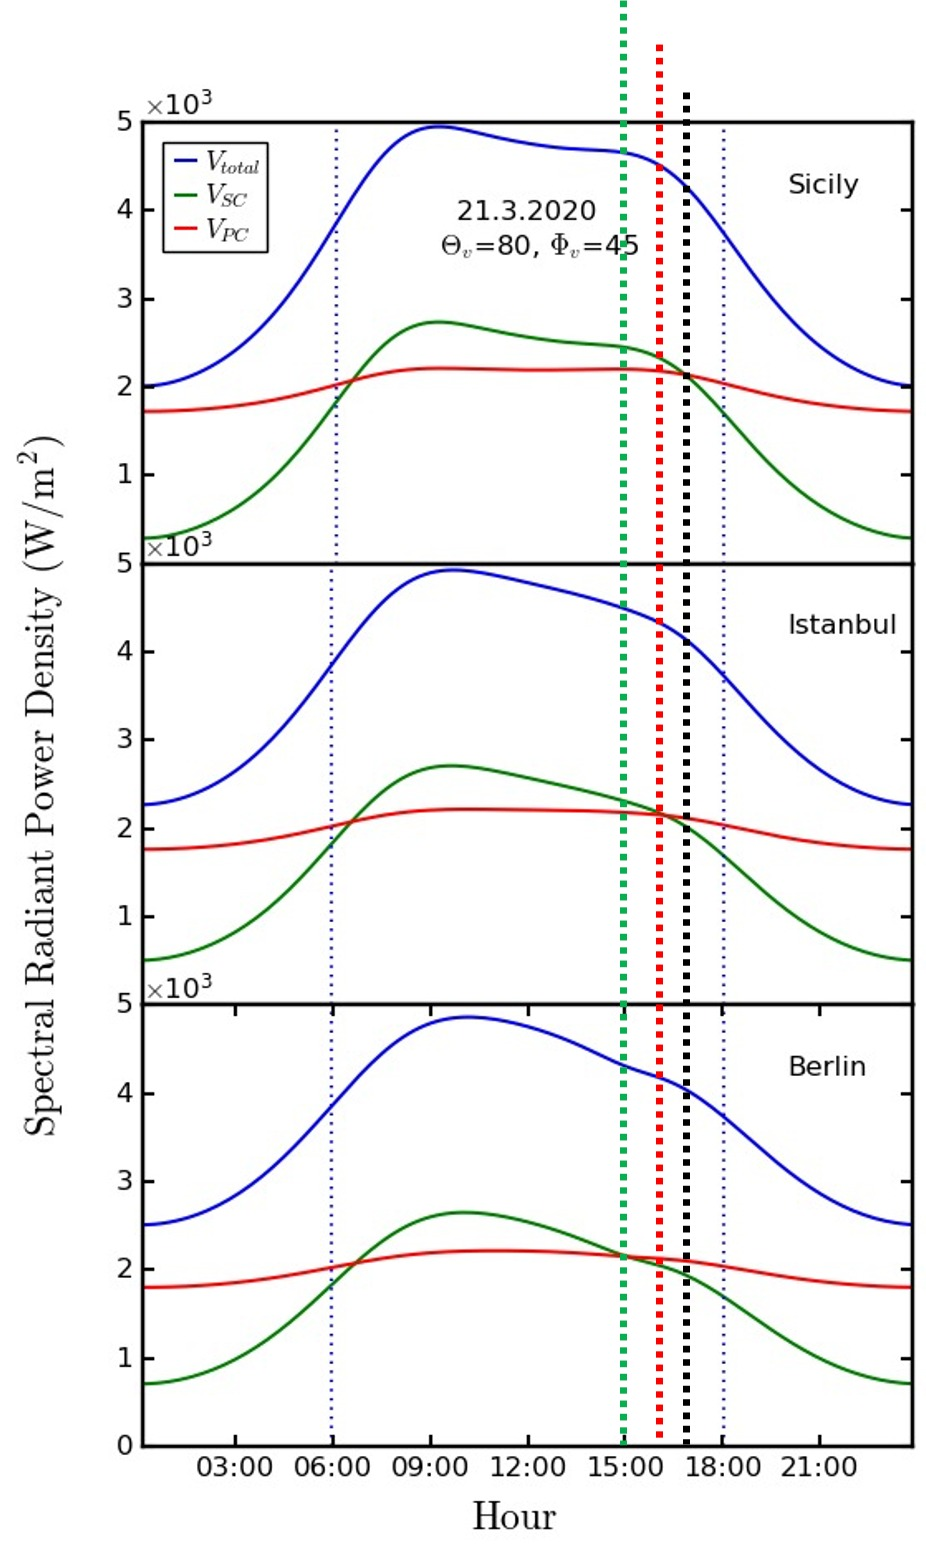
\includegraphics[width=\linewidth]{figure3}
\caption{Total (blue), scotopic (green) and photopic (red) power density as a function of time, for Sicily (\textbf{upper panel}), \.Istanbul (\textbf{middle panel}), and Berlin (\textbf{lower panel}). Vertical dashed lines indicate a possible onset of the sundowning period.\label{fig3}}
\end{figure}
\unskip

The main results of our calculations are shown in Figure~\ref{fig3} in the well-known formalism of physics and biology introduced above. The solid blue line illustrates the total vision power density versus time for three different sites, Sicily (upper panel), \.Istanbul (middle panel) and Berlin (lower panel), for a fixed view angle ($45^{\circ}$ to the south and $80^{\circ}$ above the horizon) and a turbidity of 2 (very clear sky). Photopic and scotopic sensitivities are shown by solid red and green lines. The vertical dashed lines show the transition time from photopic to scotopic vision. One can see that, depending on where you are, the crossover happens at different times.

The vertical dotted lines represent the transition of vision when different dominant cells are active. The leftmost vertical line shows where the photopic cells are more active and provide day vision. Then, at later hours, vision shifts from photopic to scotopic vision. The red dotted vertical line is our estimate of having sundowning syndrome, while at this mesopic interval our eyes cannot distinguish the colours very well. This case causes a loss of visual perception, and with that an orientational loss. This can lead to increased depression or agitation in older adults with dementia or Alzheimer's disease as reported in the literature \citep{gallagher1992}.

\section{Materials and Methods}

In the next subsections, we briefly reintroduce well-established astronomical and mathematical physical theories about solar radiation. We then discuss semi-empirical results of evolutionary biology and physiology of vision. Finally, we use these results to quantitatively model visual perception as a function of solar time and compare them to clinical observations.

\subsection{Astronomy}

In this subsection, we give a brief description of the motion of the Sun in the sky. We begin with the rotation of the Earth and its declination to the plane of the solar orbit. The declination angle is expressed by
\begin{equation}
\delta(n) \simeq 23.45^{\circ} \sin\!\left[\frac{360^{\circ}}{365}\,(284 + n)\right],
\end{equation}
where $n$ is an integer number determining the day, starting from the 1st of January ($n = 1$) and ending at the 31st of December ($n = 365$). A year is assumed to be 365 days long. The pre-factor $360^{\circ}$ is derived from dividing a unit circle by the angle in degrees. Seasons are formed due to the declination angle. Earth turns, giving us days and nights. To obtain a relation between our geometrical position and time, a solar time has to be introduced:
\begin{equation}
\mathrm{ST}(n) = \mathrm{STD}_{T} + \frac{4\,(L_{\mathrm{STD}} - L_{T}) - E(n)}{60},
\end{equation}
where $\mathrm{STD}_{T}$ is the standard time and is a function of the day of the year ($n$). Here $L_{\mathrm{STD}}$ is the longitude of the standard-time meridian (in degrees), $L_{T}$ is the local longitude and $E(n)$ is the correction due to the elliptic orbit of the Sun. A day is about 24 hours. The correction to time is given by
\begin{adjustwidth}{-\extralength}{0cm}
\begin{equation}
E(n) \simeq 229.2 \left[ 7.5\times10^{-5} + 1.868\times10^{-3}\cos B(n) - 3.2077\times10^{-2}\sin B(n) - 1.4615\times10^{-2}\cos 2B(n) - 4.089\times10^{-2}\sin 2B(n) \right],
\end{equation}
\end{adjustwidth}
where $B(n) = \frac{360^{\circ}}{365}\,(n - 1)$. A simpler expression depending on the eccentricity is given in Ref.~\citep{preetham1999}. The hour angle gives the corrected time independent of location:
\begin{equation}
\omega(n) = 15^{\circ}\left[\mathrm{ST}(n) - 12\right],
\end{equation}
taking values in the range $-180^{\circ} \le \omega(n) \le 180^{\circ}$, negative before solar noon. Next we find the position of the Sun from the sun altitude,
\begin{equation}
\alpha(\phi, \delta, \omega) = \arcsin\left[\cos\phi \cos\delta \cos\omega + \sin\phi \sin\delta\right],
\end{equation}
measuring the Sun's altitude above the horizon, where $\phi$ is the local latitude. The solar azimuth is given as
\begin{equation}
\sin\gamma(\delta, \omega, \alpha) = \frac{\cos\delta \sin\omega}{\cos\alpha},
\end{equation}
which finds the Sun in the East--West direction. The solar zenith angle $\theta_{Z}$ is the complement to $90^{\circ}$ of the solar altitude angle:
\begin{equation}
\theta_{Z}(\phi, \delta, \omega) = 90^{\circ} - \alpha = \arccos\left[\cos\phi \cos\delta \cos\omega + \sin\phi \sin\delta\right].
\end{equation}
The hour angle at sunset (and sunrise) can be found by setting the zenith angle equal to $90^{\circ}$:
\begin{equation}
\cos\omega_{s}(n) = -\tan\phi \, \tan\delta,
\end{equation}
and the length of day by
\begin{equation}
N = \frac{2}{15}\arccos\left(-\tan\phi \, \tan\delta\right).
\end{equation}

We now have to find the mean radiation coming from the Sun, which is a function of the distance from Earth to the Sun $D = 150 \times 10^{9}$~m, the radius of the Sun $R = 696 \times 10^{6}$~m, the temperature $T = 5785$~K and the Stefan--Boltzmann constant $\sigma = 5.67 \times 10^{-8}$~W\,m$^{-2}$\,K$^{-4}$:
\begin{equation}
G_{sc} = \sigma T^{4} \left(\frac{R}{D}\right)^{2} = 1367~\mathrm{W/m^{2}}.
\end{equation}
Since $D$ depends on the day of the year, the mean value outside the atmosphere is
\begin{equation}
G_{on}(n) = G_{sc}\left[1 + 0.033\cos\left(\frac{360^{\circ} n}{365}\right)\right].
\end{equation}
The extraterrestrial radiation at the surface tangent is
\begin{equation}
G_{ER}(n, \delta, \omega, \phi) = G_{on}(n)\left[\cos\phi \cos\delta \cos\omega + \sin\phi \sin\delta\right].
\end{equation}
We compute the time-wise radiation by integrating between hour angles $\omega_{2}$ and $\omega_{1}$, which yields
\begin{adjustwidth}{-\extralength}{0cm}
\begin{equation}
I_{0} = \frac{12 \times 3600}{\pi}\, G_{on} \left[\cos\phi \cos\delta \left(\sin\omega_{2} - \sin\omega_{1}\right) + \frac{\pi\left(\omega_{2} - \omega_{1}\right)}{180}\sin\phi \sin\delta\right].
\end{equation}
\end{adjustwidth}

\subsection{Electromagnetism and Quantum Theory}

Rayleigh scattering is light scattering by molecules in the atmosphere:
\begin{equation}
\beta(\lambda) \propto \frac{1}{\lambda^{4}}.
\end{equation}
The spectral intensity of the solar radiation at wavelength $\lambda$ is given by the Planck radiation law,
\begin{equation}
I_{\lambda} = \frac{8\pi h c}{\lambda^{5}}\,\frac{1}{\exp\!\left(\dfrac{hc}{\lambda k_{B} T}\right) - 1},
\end{equation}
where $h$ is Planck's constant, $k_{B}$ is Boltzmann's constant, $c$ is the speed of light in vacuum, and $T \simeq 5785$~K is the temperature of the surface of the Sun \citep{shankar1994,griffiths2017}.

\subsection{Human Vision Physiology}

The human brain and its mutual extension, the eye, are among the most complicated biological mechanisms in nature, as far as structure, physical properties and information processing are concerned. Some animal species may have better vision than humans under certain conditions (e.g., night vision or ultraviolet detection), but the human visual cortex can process information more efficiently than the visual cortex of non-human animals \citep{hubel1977,vanessen1992}. This visual dominance is generally thought to be an evolutionary product which enhanced our spatial outlook, visual acuity and trichromatic colour perception.

In our retina, there are two main functional regions packed with specialised photoreceptor cells. The fovea centralis is concentrated on the optical centre and the peripheral retina encircles the inner posterior surface of the eye. There are two types of photoreceptors: scotopic cells (rods), which are responsible for dim-light, achromatic vision, and photopic cells (cones), responsible for colour vision and high visual acuity in bright light. The fovea is rich in photopic cone cells, and scotopic rod cells are mostly distributed in the extrafoveal retina \citep{curcio1990}.

Phototransduction at the molecular scale proceeds as follows. An incoming photon hits photopigments (rhodopsin in rods, photopsins in cones). The chromophore retinal absorbs a photon and undergoes an 11-\textit{cis} to all-\textit{trans} conformational isomerism, which initiates a biochemical cascade that hyperpolarises the membrane of the photoreceptor and transmits electrical signals to the downstream retinal circuitry and the optic nerve \citep{pugh1993,baylor1996}.

\subsection{Photoreceptor Properties and Spectral Response}

Scotopic and photopic cells have very different spectral sensitivities and operating light levels:

\begin{itemize}
\item Scotopic vision (rods): rods have maximal spectral sensitivity at lower wavelengths ($\lambda_{\max} \approx 500$~nm, bluish-green), so are better able to detect in ambient darkness;
\item Photopic vision (cones): the maximum spectral sensitivity of cones occurs at longer wavelengths ($\lambda_{\max} \approx 555$~nm, greenish-yellow), which is very close to the peak of the solar spectrum reaching Earth's surface \citep{stockman2000}.
\end{itemize}

This functional shift between cone sensitivity in daylight and rod sensitivity in darkness explains the Purkinje shift---the fact that red objects appear brighter in daylight. In contrast, blue-green objects appear comparatively brighter at dusk and under low ambient light \citep{purkinje1825,lamb2013}. From an evolutionary point of view, human diurnal trichromacy was adapted to daylight, and scotopic sensitivity preserved spatial orientation in mesopic and scotopic conditions.

At the level of retinal processing, signal modulation involves ON and OFF bipolar and retinal ganglion cell (RGC) pathways. ON-centre cells depolarise when exposed to light and send signals to the brain, whereas OFF-centre cells depolarise in the absence of light \citep{werblin1969,masland2012}. This antagonistic centre--surround arrangement enhances contrast detection over a wide range of light intensities in day and night.

Human cones are specialised into three spectral subtypes in terms of photopic colour vision:
\begin{enumerate}
\item short-wavelength-sensitive (S/blue, $\lambda_{\max} \approx 420$~nm);
\item middle-wavelength-sensitive (M/green, $\lambda_{\max} \approx 530$~nm);
\item long-wavelength-sensitive (L/red, $\lambda_{\max} \approx 560$~nm).
\end{enumerate}

These cones are present in approximate relative proportions of 1:4:3 (S:M:L) in the human retina, although L-to-M ratios vary widely between individuals, as shown in Figure~\ref{fig1} \citep{roorda1999}. Evolutionary genetic studies suggest that dichromacy was the ancestral condition in catarrhine primates. The ancestral dichromacy was transformed to trichromatic vision by an X-linked duplication of the opsin gene approximately 30 to 40 million years ago, producing the M and L opsins, which facilitated the discovery of ripe foliage and fruit against green forest backgrounds \citep{dulai1999,surridge2003,hunt2017}.

\subsection{Retinal Input to Circadian Pathways: Sundowning Syndrome and SAD}

Retinal physiology also directly regulates internal biological timing (circadian rhythms) in addition to the classical image-forming vision mediated by rods and cones. This non-image-forming visual system is mediated by a third class of photoreceptors, intrinsically photosensitive retinal ganglion cells (ipRGCs), which express the photopigment melanopsin ($\lambda_{\max} \approx 480$~nm, short wavelength blue light) \citep{berson2002,hattar2002}.

The ipRGCs project directly to the hypothalamic suprachiasmatic nucleus (SCN) via the retinohypothalamic tract (RHT). The SCN, in the hypothalamus, is the master circadian pacemaker in mammals. Pineal melatonin secretion and systemic circadian synchronisation are regulated by exposure to solar light, especially seasonal photoperiod variations \citep{czeisler1999,schmidt2011}.

Disruptions in this photic entrainment pathway have been implicated in circadian and mood disorders:

\begin{enumerate}
\item Seasonal affective disorder (SAD): reduced duration of ambient light during fall and winter seasons alters ipRGC-mediated signalling to the SCN, resulting in circadian phase delays, dysregulated melatonin clearance, and reduced serotonergic tone. Certain genetic variants of the human melanopsin gene (\textit{OPN4}) have been associated with individual susceptibility to SAD \citep{roecklein2009,legates2014,ziolkowska2024}.
\item Sundowning syndrome: a common feature of neurodegenerative diseases such as Alzheimer's disease, sundowning is characterised by neuropsychiatric agitation and confusion that occurs as the day transitions into the late afternoon or evening hours. The loss of ipRGCs with age and neurodegeneration, and the consequent decrease in retinal light sensitivity \citep{lax2019,fountain2023}, affect SCN stability during twilight lighting transitions.
\end{enumerate}

\section{Conclusions}

To summarise, we have presented a quantitative physical model linking solar geometry, atmospheric spectral scattering and retinal physiology to explain the daily onset of sundowning syndrome (SS). Our calculations show that the transition from photopic (cone-dominated) to scotopic (rod-dominated) vision constitutes a major physiological boundary in twilight.

Since human colour discrimination, fine spatial resolution and visual acuity are based on photopic cone activation, the abrupt decline of photopic vision during twilight pushes visual processing into the mesopic regime. In this transition scotopic rod pathways dominate and colour contrast degrades rapidly. This mesopic visual shift can cause mild, transient dysphoria or fatigue in cognitively intact individuals. But in patients with neurodegenerative diseases such as Alzheimer's, who often show structural loss of intrinsically photosensitive retinal ganglion cells (ipRGCs) and a decrease in cognitive resilience, this transition leads to abrupt visual disorientation.

We conclude that the photopic to scotopic visual transition dominates the visual perception changes during late afternoon and early evening hours, and serves as a primary physical trigger for sundowning behaviours. Our model identifies the precise timing of this mesopic threshold for different latitudes and seasons, thus providing a foundation for targeted therapeutic interventions. These could include personalised ambient lighting protocols that attenuate the photopic-to-scotopic transition in clinical settings.

\vspace{6pt}

\authorcontributions{E.C.A. did the calculations and wrote the paper. A.S. conceived the idea, supervised the study and secured the funding, and wrote the paper. All authors have read and approved the final version of the manuscript.}

\funding{This research received no external funding.}

\institutionalreview{Not applicable.}

\informedconsent{Not applicable.}

\dataavailability{The raw data supporting the conclusions of this article will be made available by the authors, without any reservations.}

\acknowledgments{A.S. thanks the management of the Vocational School and also collaborators from the engineering and natural sciences faculty.}

\conflictsofinterest{The authors declare no conflicts of interest.}

\begin{adjustwidth}{-\extralength}{0cm}

\reftitle{References}

\begin{thebibliography}{999}

\bibitem[Martin et al.(2000)]{martin2000}
Martin, J.; Shochat, T.; Marler, M.; Ancoli-Israel, S. Circadian rhythms of agitation in institutionalized patients with Alzheimer's disease. \textit{Chronobiol. Int.} \textbf{2000}, \textit{17}, 405--418.

\bibitem[Gallagher-Thompson et al.(1992)]{gallagher1992}
Gallagher-Thompson, D.; Brooks, J.O.; Bliwise, D.; Leader, J.; Yesavage, J.A. The relations among caregiver stress, ``sundowning'' symptoms, and cognitive decline in Alzheimer's disease. \textit{J. Am. Geriatr. Soc.} \textbf{1992}, \textit{40}, 807--810. \url{https://doi.org/10.1111/j.1532-5415.1992.tb01853.x}.

\bibitem[OECD(2020)]{oecd2020}
OECD. Elderly Population (Indicator); OECD Publishing: Paris, France, 2020. \url{https://doi.org/10.1787/8d805ea1-en}.

\bibitem[WHO(2017)]{who2017}
World Health Organization. Dementia: Fact Sheet; WHO: Geneva, Switzerland, 2017.

\bibitem[NIH(2019)]{nih2019}
National Institutes of Health. Alzheimer's Disease Fact Sheet; National Institute on Aging: Bethesda, MD, USA, 2019.

\bibitem[Burns and Iliffe(2009)]{burns2009}
Burns, A.; Iliffe, S. Alzheimer's disease. \textit{BMJ} \textbf{2009}, \textit{338}, b158. \url{https://doi.org/10.1136/bmj.b158}.

\bibitem[Larson et al.(2013)]{larson2013}
Larson, E.B.; Yaffe, K.; Langa, K.M. New insights into the dementia epidemic. \textit{N. Engl. J. Med.} \textbf{2013}, \textit{369}, 2275--2277.

\bibitem[Khachiyants et al.(2011)]{khachiyants2011}
Khachiyants, N.; Trinkle, D.; Son, S.J.; Kim, K.Y. Sundown syndrome in persons with dementia: An update. \textit{Psychiatry Investig.} \textbf{2011}, \textit{8}, 275--287. \url{https://doi.org/10.4306/pi.2011.8.4.275}.

\bibitem[Cohen-Mansfield et al.(1989)]{cohenmansfield1989}
Cohen-Mansfield, J.; Watson, V.; Meade, W.; Gordon, M.; Leeks, D.; Lawson, M.; Taylor, L. Does sundowning occur in residents of an Alzheimer's unit? \textit{Int. J. Geriatr. Psychiatry} \textbf{1989}, \textit{4}, 293--298.

\bibitem[Preetham et al.(1999)]{preetham1999}
Preetham, A.J.; Shirley, P.; Smits, B. A practical analytic model for daylight. In Proceedings of the 26th Annual Conference on Computer Graphics and Interactive Techniques (SIGGRAPH '99), Los Angeles, CA, USA, 8--13 August 1999; pp. 91--100. \url{https://doi.org/10.1145/311535.311545}.

\bibitem[Boynton(1979)]{boynton1979}
Boynton, R.M. \textit{Human Color Vision}; Holt, Rinehart and Winston: New York, NY, USA, 1979.

\bibitem[Kraft et al.(1993)]{kraft1993}
Kraft, T.W.; Schneeweis, D.M.; Schnapf, J.L. Visual transduction in human rod photoreceptors. \textit{J. Physiol.} \textbf{1993}, \textit{464}, 747--765. \url{https://doi.org/10.1113/jphysiol.1993.sp019661}.

\bibitem[Schnapf et al.(1987)]{schnapf1987}
Schnapf, J.L.; Kraft, T.W.; Baylor, D.A. Spectral sensitivity of human cone photoreceptors. \textit{Nature} \textbf{1987}, \textit{325}, 439--441. \url{https://doi.org/10.1038/325439a0}.

\bibitem[Stockman et al.(1993)]{stockman1993}
Stockman, A.; MacLeod, D.I.A.; Johnson, N.E. Spectral sensitivities of the human cones. \textit{J. Opt. Soc. Am. A} \textbf{1993}, \textit{10}, 2491--2521.

\bibitem[Cao et al.(2021)]{cao2021}
Cao, X.; Yang, Y.; Selby, C.P.; Liu, Z.; Sancar, A. Molecular mechanism of the repressive phase of the mammalian circadian clock. \textit{Proc. Natl. Acad. Sci. USA} \textbf{2021}, \textit{118}, e2021174118. \url{https://doi.org/10.1073/pnas.2021174118}.

\bibitem[Shankar(1994)]{shankar1994}
Shankar, R. \textit{Principles of Quantum Mechanics}, 2nd ed.; Plenum Press: New York, NY, USA, 1994.

\bibitem[Griffiths(2017)]{griffiths2017}
Griffiths, D.J. \textit{Introduction to Electrodynamics}, 4th ed.; Cambridge University Press: Cambridge, UK, 2017.

\bibitem[Hubel and Wiesel(1977)]{hubel1977}
Hubel, D.H.; Wiesel, T.N. Ferrier lecture: Functional architecture of macaque monkey visual cortex. \textit{Proc. R. Soc. Lond. B} \textbf{1977}, \textit{198}, 1--59.

\bibitem[Van Essen et al.(1992)]{vanessen1992}
Van Essen, D.C.; Anderson, C.H.; Felleman, D.J. Information processing in the primate visual system: An integrated systems perspective. \textit{Science} \textbf{1992}, \textit{255}, 419--423.

\bibitem[Curcio et al.(1990)]{curcio1990}
Curcio, C.A.; Sloan, K.R.; Kalina, R.E.; Hendrickson, A.E. Human photoreceptor topography. \textit{J. Comp. Neurol.} \textbf{1990}, \textit{292}, 497--523.

\bibitem[Pugh and Lamb(1993)]{pugh1993}
Pugh, E.N.; Lamb, T.D. Amplification and kinetics of the activation steps in phototransduction. \textit{Biochim. Biophys. Acta} \textbf{1993}, \textit{1141}, 111--149.

\bibitem[Baylor(1996)]{baylor1996}
Baylor, D.A. How photons start vision. \textit{Proc. Natl. Acad. Sci. USA} \textbf{1996}, \textit{93}, 560--565.

\bibitem[Stockman and Sharpe(2000)]{stockman2000}
Stockman, A.; Sharpe, L.T. The spectral sensitivities of the middle- and long-wavelength-sensitive cones derived from measurements in observers of known genotype. \textit{Vision Res.} \textbf{2000}, \textit{40}, 1711--1737.

\bibitem[Purkinje(1825)]{purkinje1825}
Purkinje, J.E. \textit{Beobachtungen und Versuche zur Physiologie der Sinne}; Reimer: Berlin, Germany, 1825.

\bibitem[Lamb(2013)]{lamb2013}
Lamb, T.D. Evolution of phototransduction, vertebrate photoreceptors and retina. \textit{Prog. Retin. Eye Res.} \textbf{2013}, \textit{36}, 52--119.

\bibitem[Werblin and Dowling(1969)]{werblin1969}
Werblin, F.S.; Dowling, J.E. Organization of the retina of the mudpuppy, \textit{Necturus maculosus}. II. Intracellular recording. \textit{J. Neurophysiol.} \textbf{1969}, \textit{32}, 339--355.

\bibitem[Masland(2012)]{masland2012}
Masland, R.H. The neuronal organization of the retina. \textit{Neuron} \textbf{2012}, \textit{76}, 266--280.

\bibitem[Roorda and Williams(1999)]{roorda1999}
Roorda, A.; Williams, D.R. The arrangement of the three cone classes in the living human eye. \textit{Nature} \textbf{1999}, \textit{397}, 520--522.

\bibitem[Dulai et al.(1999)]{dulai1999}
Dulai, K.S.; von Dornum, M.; Mollon, J.D.; Hunt, D.M. The evolution of trichromatic color vision by opsin gene duplication in New World and Old World primates. \textit{Genome Res.} \textbf{1999}, \textit{9}, 629--638.

\bibitem[Surridge et al.(2003)]{surridge2003}
Surridge, A.K.; Osorio, D.; Mundy, N.I. Evolution and selection of trichromatic vision in primates. \textit{Trends Ecol. Evol.} \textbf{2003}, \textit{18}, 198--205.

\bibitem[Hunt et al.(2017)]{hunt2017}
Hunt, D.M.; Peichl, L.; Jacobs, G.H. The genetic and evolutionary bases of primate colour vision. \textit{Front. Ecol. Evol.} \textbf{2017}, \textit{5}, 34.

\bibitem[Berson et al.(2002)]{berson2002}
Berson, D.M.; Dunn, F.A.; Takao, M. Phototransduction by retinal ganglion cells that set the circadian clock. \textit{Science} \textbf{2002}, \textit{295}, 1070--1073.

\bibitem[Hattar et al.(2002)]{hattar2002}
Hattar, S.; Liao, H.W.; Takao, M.; Berson, D.M.; Yau, K.W. Melanopsin-containing retinal ganglion cells: Architecture, projections, and intrinsic photosensitivity. \textit{Science} \textbf{2002}, \textit{295}, 1065--1070.

\bibitem[Czeisler et al.(1999)]{czeisler1999}
Czeisler, C.A.; Duffy, J.F.; Shanahan, T.L.; Brown, E.N.; Mitchell, J.F.; Rimmer, D.W.; Ronda, J.M.; Silva, E.J.; Allan, J.S.; Emens, J.S.; et al. Stability, precision, and near-24-hour period of the human circadian pacemaker. \textit{Science} \textbf{1999}, \textit{284}, 2177--2181.

\bibitem[Schmidt et al.(2011)]{schmidt2011}
Schmidt, T.M.; Chen, S.K.; Hattar, S. Intrinsically photosensitive retinal ganglion cells: Many subtypes, diverse functions. \textit{J. Physiol.} \textbf{2011}, \textit{589}, 2451--2458.

\bibitem[Roecklein et al.(2009)]{roecklein2009}
Roecklein, K.A.; Rohan, K.J.; Duncan, W.C.; Rollag, M.D.; Rosenthal, N.E.; Lipsky, R.H.; Provencio, I. Melanopsin gene variations interact with season to predict sleep onset and chronotype. \textit{J. Biol. Rhythms} \textbf{2009}, \textit{24}, 411--423.

\bibitem[LeGates et al.(2014)]{legates2014}
LeGates, T.A.; Fernandez, D.C.; Hattar, S. Light as a central modulator of circadian rhythms, sleep and affect. \textit{Nat. Rev. Neurosci.} \textbf{2014}, \textit{15}, 443--454.

\bibitem[Zi\'o{\l}kowska et al.(2024)]{ziolkowska2024}
Zi\'o{\l}kowska, M.; et al. Circadian rhythms and mood disorders: Blue light, melanopsin and ipRGC pathways. \textit{J. Affect. Disord.} \textbf{2024}, \textit{345}, 112--124.

\bibitem[Lax et al.(2019)]{lax2019}
Lax, P.; Ortu\~no-Lizar\'an, I.; G\'omez-Vicente, V.; Esquiva, G.; Cuenca, N. Photosensitive melanopsin-containing retinal ganglion cells in health and disease: Implications for circadian rhythms. \textit{Int. J. Mol. Sci.} \textbf{2019}, \textit{20}, 3164.

\bibitem[Fountain et al.(2023)]{fountain2023}
Fountain, E.A.; et al. Loss of intrinsically photosensitive retinal ganglion cells and circadian dysfunction in neurodegenerative disease. \textit{Front. Neurosci.} \textbf{2023}, \textit{17}, 1102931.

\end{thebibliography}

\PublishersNote{}
\end{adjustwidth}
\end{document}